\section{Theoretical Background}
\label{sec:theory}

\subsection{Backpropagation Network}
Backpropagation networks are multi-layer feed-forward networks with supervised learning. There is no interconnection between neurons in the same layer but layers are fully connected to each other in order to be able to do forward and backward propagation.

Each neuron disposes of a weight for each input initialized to a random value in range $<0,1>$, activation function and transfer function. The input neurons 
\subsubsection{Feedforward Propagation}
\subsubsection{Backward Propagation}


\subsection{Examon}
\label{sec:examon}
Examon framework is used for exascale monitoring of supercomputing facilities. It is built on top of MQTT protocol\cite{locke2010mqtt} which allows measured metrics to be send to a central broker where received data are processed and stored in KairosDB\cite{KAIROS} database utilizing Cassandra\cite{CASSANDRA} cluster.

\begin{figure}[ht]
    \centering
    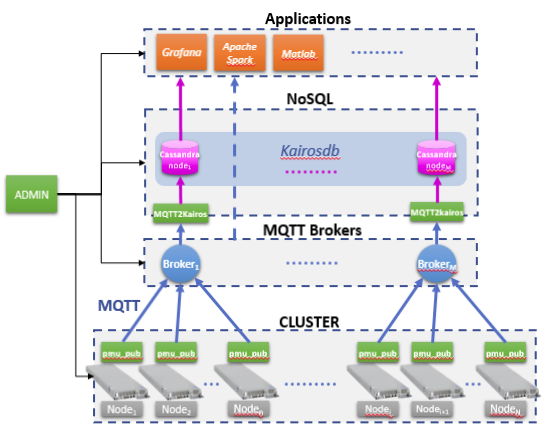
\includegraphics[width=0.5\linewidth]{examon-architecture}
    \caption{Examon framework architecture}
    \label{arch}
\end{figure}

KairosDB is used for storing metric data in time-series format whereas Cassandra, serving as a backend for KairosDB is also used for storing job-related data. More on data semantics is described in \ref{sec:data}.

